%                                                                 aa.dem
% AA vers. 9.1, LaTeX class for Astronomy & Astrophysics
% demonstration file
%                                                       (c) EDP Sciences
%-----------------------------------------------------------------------
%
%\documentclass[referee]{aa} % for a referee version
%\documentclass[onecolumn]{aa} % for a paper on 1 column  
%\documentclass[longauth]{aa} % for the long lists of affiliations 
%\documentclass[letter]{aa} % for the letters 
%\documentclass[bibyear]{aa} % if the references are not structured 
%                              according to the author-year natbib style

%
\documentclass{aa}  

%
\usepackage{graphicx}
%%%%%%%%%%%%%%%%%%%%%%%%%%%%%%%%%%%%%%%%
\usepackage{txfonts}
%%%%%%%%%%%%%%%%%%%%%%%%%%%%%%%%%%%%%%%
\usepackage{hyperref}

\usepackage{xcolor}
% To add links in your PDF file, use the package "hyperref"
% with options according to your LaTeX or PDFLaTeX drivers.
%
%own commands
\newcommand{\eq}[1]{\begin{equation}  #1 \end{equation}}
\newcommand{\eqnn}[1]{\[   #1 \]}
\newcommand{\eqa}[1]{\begin{align}   #1 \end{align}}
\newcommand{\items}[1]{\begin{itemize} #1 \end{itemize}}
\newcommand{\br}[1]{\left( #1 \right)}
\newcommand{\bc}[1]{\left\{ #1 \right\}}
\newcommand{\bb}[1]{\left[ #1 \right]}
\newcommand{\ba}[1]{\left\langle #1 \right\rangle}
\newcommand{\bs}[1]{\left| #1 \right|}
\newcommand{\cond}[1]{\left\{ \begin{matrix} #1 \end{matrix} \right.}
\newcommand{\nn}{\nonumber}
\newcommand{\nt}{\noindent}
\newcommand{\dd}{{\rm d}}
\newcommand{\mx}[1]{\mathbfss{#1}}
\newcommand{\mxg}[1]{\mbox{\boldmath{$#1$}}}
\newcommand{\expo}[1]{~{\rm e}^{ #1 }}
\newcommand{\vek}[1]{\mbox{\boldmath $#1$}}
\newcommand{\svek}[1]{\mbox{\boldmath \scriptsize $#1$}}  %small vectors
\newcommand{\ic}{{\rm i}}
\newcommand{\pr}{{\rm Pr}}
\newcommand{\refmark}[1]{\textbf{#1}}

\begin{document} 
\defcitealias{hildebrandt18}{H20}

   \title{The weak lensing likelihood in the presence of photometric redshift uncertainty}

 %  \subtitle{}

   \author{B. St\"olzner
             \inst{1},
             B. Joachimi
             \inst{1},
             A. Korn
             \inst{1},
          \and
          others
          }

   \institute{Department of Physics and Astronomy, University College London, Gower Street, London WC1E 6BT, UK\\
              \email{b.joachimi@ucl.ac.uk}
         \and
             etc.
             }

   \date{Received ; accepted }

 \abstract{TBD}  %{}{}{}{} 
% 5 {} token are mandatory

   \keywords{TBD}

   \maketitle
%
%-------------------------------------------------------------------

\section{Introduction}
Weak gravitational lensing by the large scale structure of the universe (cosmic shear) is a powerful probe of cosmology. This field is making rapid progress thanks to current and upcoming dedicated surveys, which allow to test the predictions of the standard $\Lambda$CDM cosmological model. In particular, these surveys constrain key parameters like the Hubble constant, the matter density, and the amplitude of the matter power spectrum to unprecedented precision. The main observable of weak lensing experiments are distortions in the images of background galaxies, which are observed statistically from large samples of galaxies.

 In order to theoretically model the observed signal a precise calibration of the source redshift distribution is required. Surveys typically observe millions of galaxies which are divided into several tomographic redshift bins. Given the large number of sources a complete spectroscopic redshift measurement is infeasible and therefore the redshift distribution is estimated from photometry. Several methods of photometric redshift calibration have been developed, such as direct calibrations with spectroscopic subsamples that are representative of the full sample or angular cross-correlation measurements with spectroscopic catalogues that overlap in redshift. However, it is not only crucial to adopt a calibration method that estimates the true redshift distribution as precisely as possible, but also to choose a model that is flexible enough to describe the redshift distribution accurately. Furthermore, such a model should allow us to propagate the uncertainties on the redshift distribution into the actual cosmic shear analysis. 
 
 Recently, \cite{2020MNRAS.491.4768R} applied hierarchical logistic Gaussian processes as a method to calibrate redshift distribution of galaxy samples using cross-correlation measurements with overlapping spectroscopic samples. Gaussian processes are nonparametric, i.e. they are not limited by a functional form, and therefore they fulfil the condition of being able to accurately fit the redshift distribution. However, since a gaussian process is an infinite collection of random variables, an implementation of the gaussian process into the weak lensing likelihood with fit parameters acting as nuisance parameters and subsequent marginalisation proves to be a challenging task. Therefore it is advantageous to parametrise the redshift distribution using a model with a finite number of free parameters and enough flexibility to fit the actual data properly.

In this paper we present a parametrisation of the redshift distribution of samples of galaxies as a 'comb', i.e. a modified gaussian mixture model with fixed, equidistant separation between components, an identical variance, and a fixed number of components. The amplitudes of each gaussian component serve as fit parameters in the redshift distribution calibration. We implement this model into a weak lensing likelihood. Since our model is linear in the fit parameters we can analytically marginalise over the fitted amplitudes. The advantage of this procedure is that we can use a large number of components to fit the redshift distribution which gives the model enough flexibility to fit a potentially complex redshift distribution. At the same time we do not increase the total number of free parameters of the likelihood, so that it is still feasible to sample the likelihood via MCMC without a significant increase in runtime. Additionally, the correlation between fit parameters is fully propagated into the likelihood.
We test our model by analysing cosmic shear data from KiDS  \citep[Kilo Degree Survey;][]{2015MNRAS.454.3500K,2015A&A...582A..62D,2017A&A...604A.134D} and VIKING \citep[VISTA Kilo-Degree Infrared Galaxy Survey;][]{2013Msngr.154...32E}. In particular, we analyse the dataset of \cite{hildebrandt18} by fitting the comb model to the redshift distribution histograms that were calibrated using a weighted direct calibration with deep spectroscopic catalogues.
However, our model has a disadvantage compared to the cosmic shear analysis of  \cite{hildebrandt18}: When modelling the 2-point shear correlation function, the authors introduce nuisance parameters with gaussian priors that linearly shift the precalibrated redshift distribution of each tomographic bin. These shifts represent the uncertainties in the photometric redshift calibration, which are marginalised when sampling the likelihood via MCMC. A linear shift does not capture the full variance of the redshift distribution, which is why it particularly interesting to study a model that integrates the full variance. Including nuisance parameters that shift the redshift distribution allows for an additional self-calibration of the redshift distribution using cosmic shear data. While in principle we could do the same procedure with the comb model of the redshift distribution, this is infeasible in practice because of the large number of parameters that characterise the redshift distribution which is why we choose to analytically marginalise over these parameters. In order to allow the cosmic shear data to calibrate the redshift distribution we adopt a second calibration step: after fitting the comb model to the redshift histograms we apply an iterative fitting method of both cosmological and nuisance parameters. The best-fit nuisance parameters then represent a model of the redshift distribution calibrated both with deep spectroscopic catalogues and cosmic shear data. When sampling the cosmological parameters we marginalize over this set of nuisance parameters.
 
The paper is structured as follows: In Sect. \ref{sec:data} the data products are described. The redshift distribution model is described in Sect \ref{sec:comb} and the theoretical modelling of the cosmic shear signal with analytic marginalisation over nuisance parameters is described in Sect \ref{sec:likelihood}. In Sect. \ref{sec:calibration} the redshift distribution calibration is described. Results are presented in Sect. \ref{sec:results} and discussed in Sect. \ref{sec:discussion}.
 
%--------------------------------------------------------------------
\section{Data}
\label{sec:data}
In this section we summarise the cosmic shear dataset that is analysed in Sect. \ref{sec:results}.
We use data from the European Southern Observatory's Kilo Degree Survey \citep[KiDS; ][]{2015MNRAS.454.3500K,2015A&A...582A..62D,2017A&A...604A.134D} and the fully overlapping VISTA Kilo-Degree Infrared Galaxy Survey \citep[VIKING; ][]{2013Msngr.154...32E}. This data set, dubbed KV450, combines optical and near infrared data on 450 ${\rm deg}^2$. The photometric redshift calibration is greatly improved compared to the earlier KiDS data set \citep{2017MNRAS.465.1454H} thanks to the addition of five near-infrared bands from VIKING that complement the four optical bands from KiDS. These additional bands greatly improve the accuracy of photometric redshifts, which are essential for cosmic shear measurements. The fiducial technique of redshift calibration utilises a weighted direct calibration of five tomographic bins with deep spectroscopic catalogues (DIR). Uncertainties on the redshift distribution are estimated by a spatial bootstrapping method. The robustness of the photometric redshift calibration has been tested by excluding certain catalogues from the calibration sample as well as using alternative calibration samples. Additionally, the angular cross-correlation between KV450 galaxies and spectroscopic calibration samples has been studied as an alternative to the fiducial direct weighted calibration.

In the fiducial KV450 cosmic shear analysis, presented in \cite{hildebrandt18}, the combined KiDS+VIKING data set \citep{2019A&A...632A..34W} is binned into five tomographic redshift bins based on their most probable Bayesian redshift $z_B$, inferred with the photo-z code {\sc BPZ} \citep{2000ApJ...536..571B}. Four bins of width $\Delta z = 0.2$ in the range $0.1 < z_{\rm B} <0.9$ and a fifth bin with $0.9 < z_{\rm B} < 1.2$ are defined and calibrated using the aforementioned direct calibration method. The photometric redshift distribution is then used to model the 2-point shear correlation function and constraints on cosmological parameters are derived using an MCMC sampling of the weak lensing likelihood. 

In our analysis we use the same data set that was analysed in \cite{hildebrandt18}, i.e. the redshift distribution histograms in five tomographic bins with the corresponding covariance matrix between redshift bins and the 2-point shear correlation function measurements.

%these uncertainties are taken into account by introducing nuisance parameters that linearly shift the redshift distribution of each tomographic bin when modelling the 2-point shear correlation functions.  However, linear shifts of the redshift distribution do not capture the full variance of the distributions and therefore it is worth testing to what extent the particular choice of nuisance parameters has an impact on the inferred constraints on cosmological parameters.The redshift distribution of each bin was inferred using the fiducial direct calibration method with deep spectroscopic surveys (DIR) which also provides a covariance matrix that was estimated from a bootstrap analysis. The observable used in the likelihood analysis is the 2-point shear correlation function $\xi(\theta)$ between tomographic bins.
\section{Redshift distribution model}
\label{sec:comb}
We model the redshift distribution of each tomographic bin $\alpha$ as a 'comb', i.e. a slightly modified Gaussian mixture with $N_z$ components per bin, with fixed, equidistant separation between the components, and with identical variance $\sigma_{\rm comb}^2$ on which the resulting posterior is conditioned (i.e. it is optimised but then fixed). Hence,
\eq{
p^{(\alpha)}(z) = \sum_{i=1}^{N_z} A_i^\alpha\; {\cal K}\br{z; z_i, \sigma_{\rm comb}^2}\;,
}
where the only free parameters to be fitted are the amplitudes $A_i^\alpha$. We choose to model the normalised 'teeth' of the comb as
\eq{
{\cal K} \br{z; z_i, \sigma_{\rm comb}^2} = \frac{z}{N(z_i, \sigma_{\rm comb})}\, \exp \bc{- \frac{(z-z_i)^2}{2 \sigma_{\rm comb}^2} }\;, 
}
with normalisation over the interval $\bb{0;\infty}$
\eq{
N(z_i, \sigma_{\rm comb}) = \sqrt{\frac{\pi}{2}}\, z_i\, \sigma_{\rm comb}\; {\rm erfc} \br{-\frac{z_i}{\sqrt{2} \sigma_{\rm comb}}} + \sigma^2 \exp \bc{-\frac{z_i^2}{2 \sigma_{\rm comb}^2}}.
}
Note that the method does not depend on a particular choice of ${\cal K}$. This form has the advantage of ensuring $p^{(\alpha)}(0)=0$. The redshift distribution is normalised, so that
\eq{
\sum_{i=1}^{N_z} A_i^\alpha = 1\;.
}
which leads to
\eqa{
p^{(\alpha)}(z) &= {\cal K}\br{z; z_{N_z}, \sigma_{\rm comb}^2} \\ \nn
& ~~~~+ \sum_{i=1}^{N_z-1} A_i^\alpha \bb{ {\cal K}\br{z; z_i, \sigma_{\rm comb}^2}  - {\cal K}\br{z; z_{N_z}, \sigma_{\rm comb}^2} } \\ \nn
&\equiv \sum_{i=1}^{N_z} A_i^\alpha p_i(z)\;,
}
where $A_{N_z}^\alpha =1$ is fixed. Since the amplitudes should be positive, it is convenient to define
\eq{
a_i^\alpha \equiv \ln A_i^\alpha\;
}
as the actual fit parameters. The final result of the redshift calibration procedure with data $\boldsymbol{d}_{\rm cal}$ is then
\eq{
\pr \br{ \bc{a_i^\alpha} | \boldsymbol{d}_{\rm cal}} \approx {\cal N}\br{ a_i^\alpha; {a^*}_i^\alpha, \tens{\Sigma}_{\rm cal}}\;,
}
where the posterior is approximated by a multivariate Gaussian with best-fit ${a^*}_i^\alpha$ and covariance $\tens{\Sigma}_{\rm cal}$.

%By resampling $\boldsymbol{d}_{\rm cal}$ using the full covariance matrix of the five tomographic bins and refitting the amplitudes of the gaussians we infer the covariance matrix $\tens{\Sigma}_{\rm cal}$ for the amplitudes.


%-------------------------------------------------------------------
\section{Theoretical modelling of the cosmic shear signal}
\label{sec:likelihood}
In this section we describe the weak lensing likelihood and develop an analytic marginalisation over the nuisance parameters, i.e. the fitted amplitudes of the comb model.
We integrate the marginalisation procedure into the KV450 likelihood code from \cite{hildebrandt18} which is implemented in the publicly available {\sc MontePython}\footnote{\url{https://github.com/brinckmann/montepython_public}} package \citep{Audren:2012wb, Brinckmann:2018cvx}. We sample the likelihood in the {\sc MultiNest} \footnote{\url{https://github.com/farhanferoz/MultiNest}} mode \citep{feroz09,feroz19} using the python wrapper {\sc PyMultiNest} \citep{buchner14}. The matter power spectrum is estimated with the public code {\sc Class}\footnote{\url{https://github.com/lesgourg/class_public}}\citep{blas11} with non-linear corrections from {\sc HMCode} \citep{mead15}.
%-------------------------------------------------------------------
\subsection{Weak lensing likelihood}

The cosmic shear angular power spectrum between two tomographic bins $\alpha$ and $\beta$ is given by
\eqa{
C^{(\alpha \beta)}(\ell) &= \int_0^\infty \dd \chi \frac{q^{(\alpha)}(\chi) q^{(\beta)}(\chi)}{f_K^2(\chi)} P_\delta\br{\frac{\ell}{f_K(\chi)},\chi}\; \\ \nn
&= \sum_{i,j=1}^{N_z} A_i^\alpha A_j^\beta  \int_0^\infty \dd \chi \frac{q_i(\chi) q_j(\chi)}{f_K^2(\chi)} P_\delta\br{\frac{\ell}{f_K(\chi)},\chi}\; \\ \nn
&\equiv \sum_{i,j=1}^{N_z} A_i^\alpha A_j^\beta\; c^\prime_{ij}(\ell)\;,
}
where $P_\delta$ is the matter power spectrum, and $f_K$ and $\chi$ are the comoving angular diameter and radial distances, respectively. The lensing kernel $q$ is a linear functional of the corresponding redshift distribution, so that it is straightforward to extract the amplitudes of the redshift distribution model. In the final equality we have defined $c^\prime_{ij}$, which is the angular weak lensing power spectrum for two Gaussian mixture components at $z_i$ and $z_j$ as redshift distributions. The observable is usually linear transformation of the cosmic shear angular power spectrum, which we write in general form for a kernel $K$ as
\eqa{
X_l^{(\alpha \beta)} &= \int_0^\infty \frac{\dd \ell\, \ell}{2 \pi}\, K_l(\ell)\, C^{(\alpha \beta)}(\ell)\; \\ \nn
&\equiv \sum_{i,j=1}^{N_z} A_i^\alpha A_j^\beta\; c_{ij,l}\;.
\label{eq:obs}
}
Again, since the transformation is linear, we can capture the two-point statistic for Gaussian components at $z_i$ and $z_j$ in the quantity $c_{ij}$.
In particular, we are interested in the 2-point shear correlation function, which is the primary observable in the fiducial KV450 cosmic shear analysis. The 2-point shear correlation function between two tomographic bins can be modelled with spherical Bessel functions of the first kind $J_{0/4}(\ell)$ as the kernel. We find
\eqa{
\xi_\pm^{ij}(\theta) &= \int_0^\infty \frac{\dd \ell\, \ell}{2 \pi}\,J _{0/4}(\ell \theta)\, C^{(\alpha \beta)}(\ell)\\ \nn
&\equiv \sum_{i,j=1}^{N_z} A_i^\alpha A_j^\beta\; c_{ij,l}\;.
}
The Gaussian log-likelihood is then given by
\eq{
{\cal L} = \sum_{l,l',\alpha,\beta,\gamma,\delta} \Delta_l^{(\alpha \beta)}\; Z_{(l,\alpha,\beta) \,  (l',\gamma,\delta)}\; \Delta_{l'}^{(\gamma \delta)}\;,
}
where we have defined
\eq{
\Delta_l^{(\alpha \beta)} \equiv d_l^{(\alpha \beta)} - \sum_{i,j=1}^{N_z} A_i^\alpha A_j^\beta\; c_{ij,l}\;.
}
Here, $d$ denotes the element of the observed data vector. The inverse covariance, which is assumed to be cosmology-independent is given by $\tens{Z}$. We note that all cosmology dependence is in the $c_{ij,l}$.

\subsection{Marginal likelihood}

The goal is to analytically derive the likelihood of a weak lensing experiment, marginalised over the potentially large number of nuisance parameters $\boldsymbol{p}_{\rm nu}$ originating from the redshift calibration. If $\boldsymbol{p}_{\rm co}$ denote the cosmological parameters of interest, we obtain
\eq{
\pr \br{\boldsymbol{d} | \boldsymbol{p}_{\rm co}} = \int \dd^{N_{\rm nu}} p_{\rm nu}\; \pr \br{\boldsymbol{d} | \boldsymbol{p}_{\rm co}, \boldsymbol{p}_{\rm nu}} \pr \br{\boldsymbol{p}_{\rm nu}}\;,
}
where the prior on the nuisance parameters is given in this case by the posterior of the fit to the redshift distribution. The nuisance parameters are therefore the collection of amplitude parameters $\bc{a_i^\alpha}$.

In the following we will assume that the overall weak lensing likelihood is Gaussian. Moreover, we apply a Laplace approximation to the posterior in the subspace spanned by the nuisance parameters, i.e. we effectively assume the posterior to be well-represented by a Gaussian in this regime. The marginalised log-likelihood,
\eq{
{\cal L}_{\rm marg}  \equiv -2 \ln \pr \br{\boldsymbol{d} | \boldsymbol{p}_{\rm co}}\;,
}
is then given by \citep{taylor10}
\eq{
\label{eq:marginal_likelihood}
{\cal L}_{\rm marg} = {\cal L}_{\rm fid} - \frac{1}{2} \boldsymbol{\cal L^\prime}^\tau  \bb{ {\cal L^{\prime\prime}} + 2 \tens{\Sigma}^{-1}_{\rm cal} }^{-1} \boldsymbol{\cal L^\prime} + \ln \det \br{ \mathbb{I} + \frac{1}{2} {\cal L^{\prime\prime}} \tens{\Sigma}_{\rm cal}}\;,
}
where ${\cal L}_{\rm fid}$ is the log-likelihood evaluated at the best fit of the nuisance parameters,
\eq{
{\cal L}_{\rm fid} \equiv -2 \ln \pr \br{\boldsymbol{d} | \boldsymbol{p}_{\rm co}, \boldsymbol{p}^*_{\rm nu}}\;.
}
A single prime denotes the derivative of the log-likelihood with respect to the nuisance parameters, a double prime the Hessian matrix of second derivatives. All of these derivatives are to be evaluated at the best fit of the nuisance parameters. The covariance matrix of nuisance parameters, originating from the calibration of the photometric redshift distribution, is denoted by $\tens{\Sigma}_{\rm cal} $.

%-------------------------------------------------------------------
\subsection{Marginalisation over nuisance parameters}

For the specific case of marginalising over the redshift distribution nuisance parameters the vector $\boldsymbol{\cal L^\prime}$ has elements
\eqa{
\frac{\partial {\cal L}}{\partial a_m^\mu} &= \sum_{l,l',\alpha,\beta,\gamma,\delta}  \left\{ \frac{\partial \Delta_l^{(\alpha \beta)}}{\partial a_m^\mu}\; Z_{(l,\alpha,\beta) \,  (l',\gamma,\delta)}\; \Delta_{l'}^{(\gamma \delta)} \right. \\ \nn
& \hspace*{1cm} + \left. \Delta_l^{(\alpha \beta)}\; Z_{(l,\alpha,\beta) \,  (l',\gamma,\delta)}\; \frac{\partial \Delta_{l'}^{(\gamma \delta)}}{\partial a_m^\mu} \right\}\;,
}
with
\eq{
\frac{\partial \Delta_l^{(\alpha \beta)}}{\partial a_m^\mu} = - A_m^\mu \sum_i c_{im,l} \br{\delta_{\alpha \mu}\, A_i^\beta + \delta_{\beta \mu}\, A_i^\alpha}\;,
}
where $\delta_{\alpha \beta}$ denotes the Kronecker delta symbol. The Hessian matrix ${\cal L^{\prime\prime}}$ has elements
\eqa{
\label{eq:hessian}
\frac{\partial^2 {\cal L}}{\partial a_m^\mu\, \partial a_n^\nu} &= \sum_{l,l',\alpha,\beta,\gamma,\delta} 
\left\{ 
\frac{\partial \Delta_l^{(\alpha \beta)}}{\partial a_m^\mu}\; Z_{(l,\alpha,\beta) \,  (l',\gamma,\delta)}\; \frac{\partial \Delta_{l'}^{(\gamma \delta)}}{\partial a_n^\nu}  \right. \\ \nn
& \!\!\!\! + \frac{\partial \Delta_l^{(\alpha \beta)}}{\partial a_n^\nu}\; Z_{(l,\alpha,\beta) \,  (l',\gamma,\delta)}\; \frac{\partial \Delta_{l'}^{(\gamma \delta)}}{\partial a_m^\mu} 
+ \frac{\partial^2 \Delta_l^{(\alpha \beta)}}{\partial a_m^\mu\, \partial a_n^\nu}\; Z_{(l,\alpha,\beta) \,  (l',\gamma,\delta)}\; \Delta_{l'}^{(\gamma \delta)} \\ \nn
& \!\!\!\! \left. + \Delta_l^{(\alpha \beta)}\; Z_{(l,\alpha,\beta) \,  (l',\gamma,\delta)}\; \frac{\partial^2 \Delta_{l'}^{(\gamma \delta)}}{\partial a_m^\mu\, \partial a_n^\nu}
\right\}\;,
}
with 
\eqa{
\frac{\partial^2 \Delta_l^{(\alpha \beta)}}{\partial a_m^\mu\, \partial a_n^\nu} &= - A_m^\mu A_n^\nu \, c_{mn,l} \br{ \delta_{\alpha \mu} \delta_{\beta \nu} + \delta_{\beta \mu} \delta_{\alpha \nu} }\\ \nn
& ~~~~~ - \delta_{mn} \delta_{\mu \nu}\, A_m^\mu \sum_i c_{im,l} \br{\delta_{\alpha \mu} A_i^\beta + \delta_{\beta \mu} A_i^\alpha}\;.
}
For $N_{\rm bin}$ tomographic bins used in the analysis, $N_{\rm bin} \times N_z$ nuisance parameters are marginalised over (modulo those amplitudes fixed by the normalisation of the redshift distribution).


%-------------------------------------------------------------------
\subsection{A simpler approximation}

For current survey data there is very little self-calibration of redshift distributions, i.e. the likelihood in the subspace of the redshift nuisance parameters is generally quite flat. It is therefore reasonable to test a cruder approximation that assumes that the curvature of the likelihood is negligible over the prior range of the nuisance parameters. Then Eq. (\ref{eq:marginal_likelihood}) turns into
\eq{
{\cal L}_{\rm marg} \approx {\cal L}_{\rm fid} - \frac{1}{4} \boldsymbol{\cal L^\prime}^\tau  \tens{\Sigma}_{\rm cal} \boldsymbol{\cal L^\prime} \;.
}
If the calibration data best-fit coincides with the maximum of the weak lensing likelihood, the expression will reduce to ${\cal L}_{\rm fid}$, i.e. the marginal likelihood is approximated as the likelihood conditioned on the best-fit values. Broadening of the marginal likelihood only occurs if the best-fit is away from the weak lensing likelihood peak.

We can discount an even cruder approximation that also ignores the slope of the weak lensing likelihood and assumes ${\cal L}$ is constant over the allowed range of the nuisance parameters. This would imply ${\cal L}_{\rm marg} \approx {\cal L}_{\rm fid}$, which is equivalent to assuming that the calibration procedure has constrained the redshift nuisance parameters so tightly relative to the width of the weak lensing likelihood that the statistical uncertainty of the calibration procedure becomes negligible.
\section{Redshift distribution calibration}
\label{sec:calibration}
We calibrate the redshift distribution by fitting the model defined in Sect. \ref{sec:comb} to the redshift distribution histogram of \cite{hildebrandt18}. The fiducial KV450 weak lensing likelihood contains nuisance parameters $\delta z_i$, which linearly shift the mean redshift of each tomographic bin. When sampling the likelihood this then leads to a self-calibration of the redshift distribution with cosmic shear data. In our analysis these shifts get replaced by the amplitudes of the comb components, which gives the model more flexibility to match the true redshift distribution. Given the dimensionality of the new nuisance parameter space, a sampling of nuisance parameters in an MCMC becomes computationally expensive. Thus, we marginalise analytically over the uncertainties on the fitted amplitudes. By doing so, we however loose the ability to calibrate the redshift distribution with cosmic shear data since the amplitudes no longer appear as free parameters in the likelihood. In order to retain the calibration of the redshift distribution with cosmic shear data we perform an additional calibration step.

Our goal is to find the best-fit in the combined parameter space of cosmological and nuisance parameters. Given the high dimensionality of the nuisance parameter space we adopt an iterative method:

1) We fit the gaussian comb model, defined in Sect. \ref{sec:comb}, to redshift distribution histograms of \cite{hildebrandt18} which are calibrated with the fiducial DIR method. This is done by minimising 
\eq{
\chi^2 = \left(n^{\rm data}_i - n^{\rm model}_i\right) C^{-1}_{ij} \left(n^{\rm data}_j - n^{\rm model}_j\right),
} 
where $n^{\rm data}_i$ and $n^{\rm model}_i$ are the observed and modelled histogram heights in bin $i$ respectively and $C^{-1}_{ij}$ denotes the inverse covariance matrix between the histogram bins in all five tomographic redshift bins. We estimate the uncertainties on the fit parameters by resampling the data vector using a multivariate gaussian distribution from which calculate the covariance matrix $\Sigma_{\rm cal}$ of fit parameters,

2) We fix the amplitudes of the gaussian comb to the best-fit parameters found in the previous step. We then run a non-linear optimiser to find the best-fit cosmological parameters that minimise the log-likelihood given in Eq. \ref{eq:marginal_likelihood}.

3) For fixed cosmological parameters the displacement from the peak of the likelihood in nuisance parameter space is given by \citep{taylor10}:
\begin{equation}
\delta\psi_\alpha = -\mathcal{L}_\beta\left[\mathcal{L}_{\alpha\beta}+2C_{\alpha\beta}^{-1}\right]^{-1}. 
\end{equation}
Fixing the cosmological parameters to the ones found in step 2), we use Newton's method to optimise the nuisance parameters towards the peak of the likelihood.

By iterating over steps 2 and 3 both cosmological and nuisance parameters eventually converge to the global best-fit values. The best-fit nuisance parameters then represent the redshift distributions of each tomographic bin, calibrated using both spectroscopic catalogues and the actual cosmic shear data. The iterative fitting procedure is illustrated in Fig. \ref{fig:iterative_calibration}. After the calibration the redshift distributions we proceed with sampling of the likelihood in cosmological parameter space while marginalising over nuisance parameters.
\begin{figure}
\label{fig:iterative_calibration}
\centering
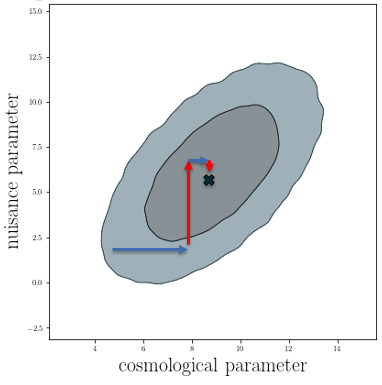
\includegraphics[scale=0.4]{plots/iterative.png}
\caption{Sketch of the iterative fitting method that is used to find the best-fit in the combined parameter space of cosmological and nuisance parameters. We alternate between optimising cosmological parameters keeping nuisance parameters fixed using a non-linear optimiser and optimising nuisance parameters using Newton's method keeping cosmological parameters fixed. After several iterations we achieve convergence to the best-fit in the combined parameter space.}
\label{fig:comb}
\end{figure}
\section{Results}
\label{sec:results}
\subsection{Redshift distribution calibration}
\label{sec:redshift_calibration}
The first step in the calibration of the KV450 redshift distribution is to fit our modified gaussian mixture model to the redshift histograms of \cite{hildebrandt18}. This fit is done simultaneously for all five tomographic redshift bins in order to account for the correlations between bins. When deriving a histogram that models the redshift distribution of galaxies in a given tomographic bin, the width of the histogram bins is a free parameter. In the fiducial analysis this bin width is set to $\Delta z = 0.05$.  To test the sensitivity of the calibration to the choice of bin width of the input data histograms, we additionally perform the calibration using a set of data histograms with a bin width of $\Delta z = 0.025$.  Since these histograms trace the same underlying redshift distribution of galaxies in each tomographic bin, the distribution inferred by fitting the comb model should not depend on the choice of binning of the input data. However, it is still to insightful to compare the fit results from these two types of input data histograms in order to test to what extent the redshift distribution calibration is affected by noise. Moreover, we are free to choose the number of gaussian components of the redshift distribution model and the variance of the components. In Appendix \ref{ap:calibration} we perform several tests, comparing different choices for the aforementioned free parameters and address their impact on the cosmological analysis. In this section we report our fiducial result using a model with $N = Y$ components and a variance of $\sigma_{\rm comb} = Y$. 
\begin{figure*}
\centering
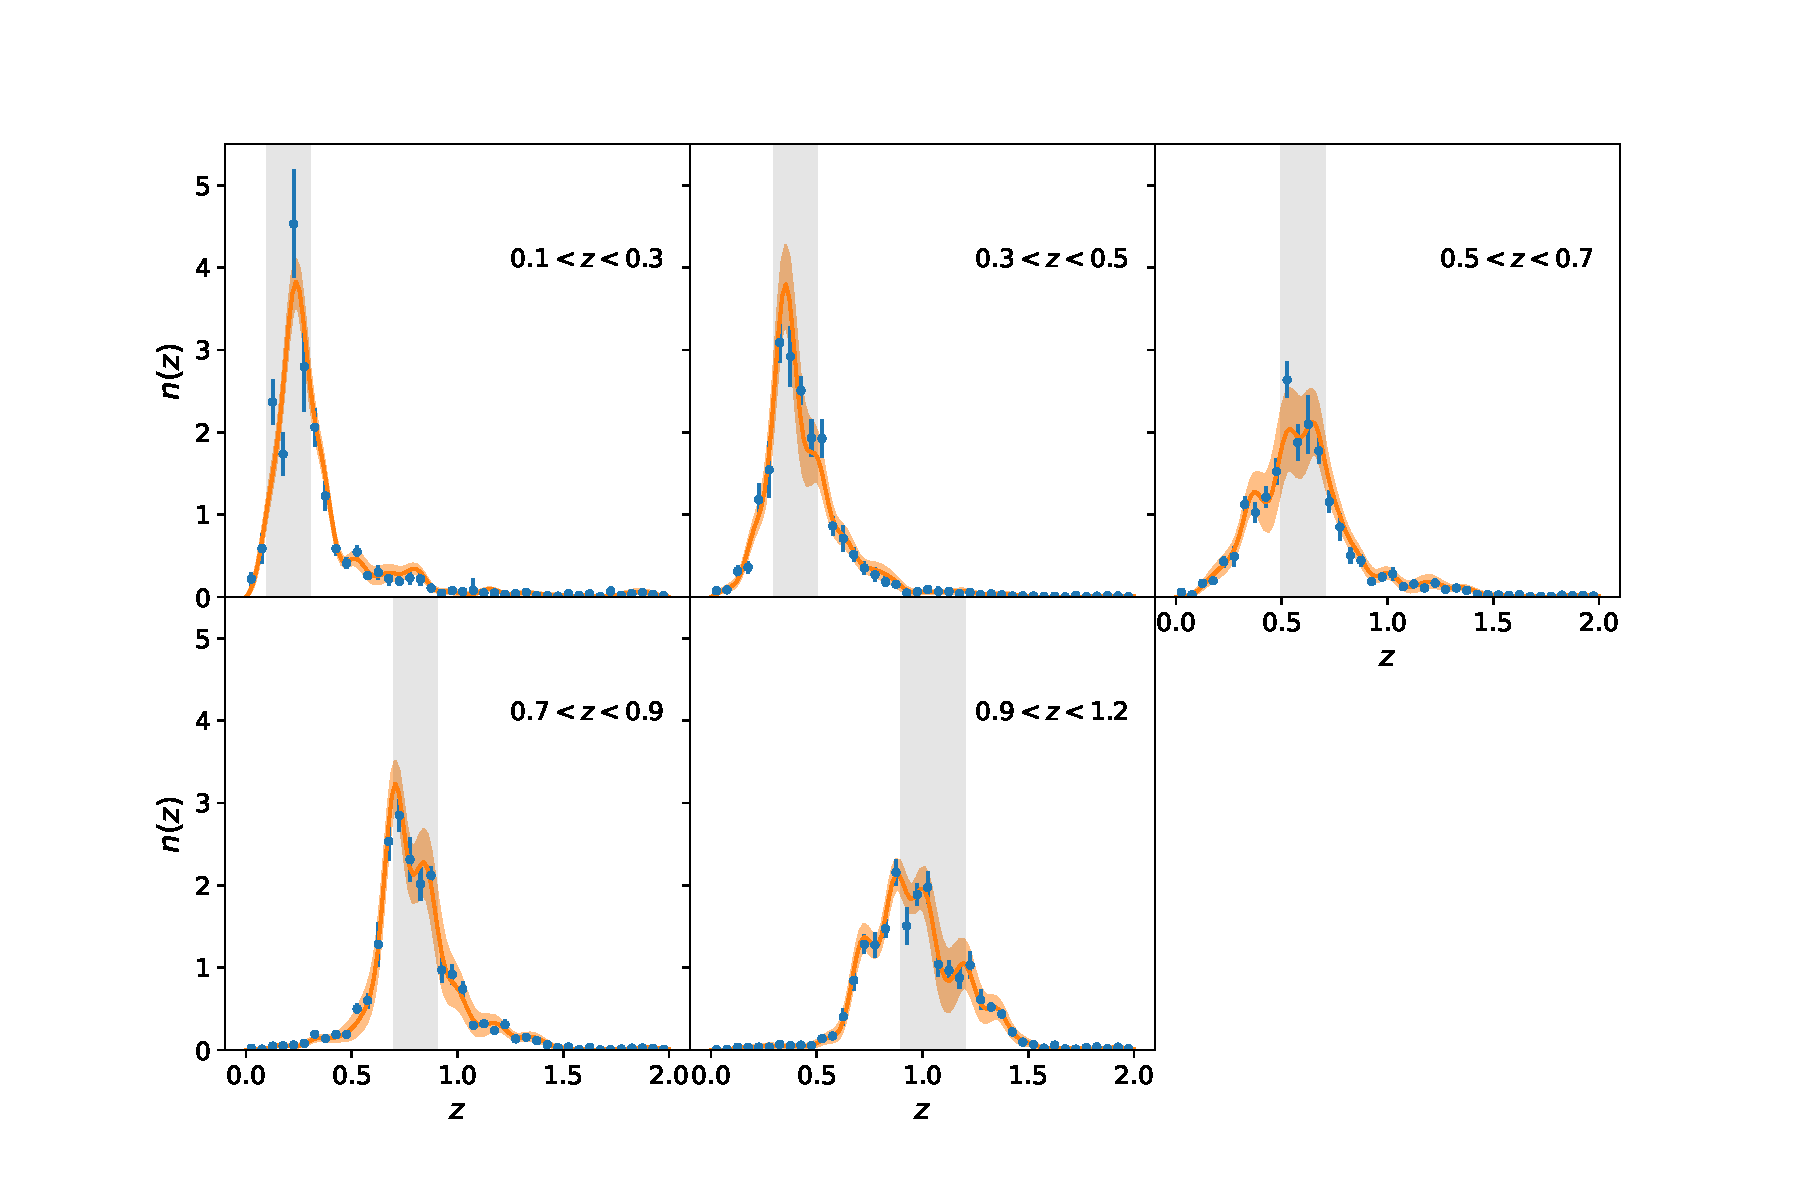
\includegraphics[width=\linewidth]{plots/combfit_linear.pdf}
\caption{Fit results of a gaussian mixture with N components to the N(z) distribution in 5 tomographic redshift bins. Data is shown in blue and the resulting fit is shown in orange with shaded region indicating the 1$\sigma$ confidence interval. {\color{red} This is a redshift distribution before iterative optimisation. Need a plot after iterative optimisation. And probably put the covariance matrix next to it}}
\label{fig:comb}
\end{figure*}
\begin{figure}
\centering
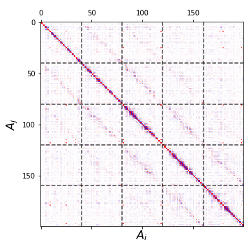
\includegraphics[scale=0.7]{plots/corr.png}
\caption{Correlation matrix of the best-fit comb amplitudes.}
\label{fig:correlation_matrix}
\end{figure}
The best-fit model is illustrated in Fig. \ref{fig:comb} and the corresponding correlation matrix  is presented in Fig. \ref{fig:correlation_matrix}, showing the correlation between the amplitudes of different tomographic redshift bins, which can also be observed in the input data covariance matrix.  

We proceed with a further calibration of the redshift distribution using the iterative fitting method of cosmological and nuisance parameters described in Sect. \ref{sec:calibration}. The fit result after each step for the three most interesting cosmological parameters $A_{IA}$, $\Omega_m$, and $S_8$ are reported in Table \ref{tab:iterative_calibration}. 
\begin{table}
\begin{tabular}{lllll}
& $A_{IA}$ & $\Omega_m$ & $S_8$ & $\chi^2$\\
\hline
\hline
fiducial KV450 likelihood & $0.8656$ & $0.2146$ & $0.7708$ & $179.8831$\\
\hline
1. cosmology optimisation & $0.7353$ & $0.2139$ & $0.7768$ & $180.67$\\
2. nuisance optimisation & --- & --- & --- & $179.105$\\
3. cosmology optimisation & $0.7903$ & $0.213$ & $0.7882$ & $178.617$\\
\end{tabular}
\caption{Results of the iterative fitting of cosmological and nuisance parameters to the KV450 cosmic shear data and comparison to the fiducial KV450 likelihood. When optimising cosmological parameters we fit $\omega_{\rm cdm}$, $\omega_{\rm b}$, $A_{\rm s}$, $n_{\rm s}$, and $h$ as well as the nuisance parameters $A_{\rm IA}$, $A_{\rm bary}$, $\delta c$, and $A_{\rm c}$. When optimising nuisance parameters we vary the amplitudes of the gaussian comb. Results are shown for the three most interesting parameters, for which the cosmic shear likelihood has the largest constraining power. We find convergence after three iterations of the calibration, resulting in a better fit to the cosmic shear data compared to the fiducial analysis.}
\label{tab:iterative_calibration}
\end{table}
The iterative optimisation method shows a fast convergence to the best-fit in the full parameter space of cosmological and nuisance parameters after only three iterations. This is expected since we start from an already well calibrated redshift distribution so that expect only small shifts of the redshift distribution. Comparing the best fit $\chi^2$ values we find that our model provides a better fit to the cosmic shear data than the fiducial KV450 model. This indicates that a linear shift of the mean of the redshift distribution indeed does not capture the full variance of the data and that it is beneficial to allow for a full shift of the redshift distribution when deriving constraints on cosmological parameters. Interestingly, we find the the matter density $\Omega_m$ does not shift significantly when switching from a linear shift of the mean of the redshift distribution to a full shift, while the values of the intrinsic alignment amplitude $A_{\rm IA}$ and $S_8$ show a more significant shift.

\subsection{Marginalisation over nuisance parameters} 
Using the redshift distribution that were calibrated in the previous section we sample the weak lensing likelihood in cosmological parameter space with analytical marginalisation over the uncertainty on the amplitudes of the fitted redshift distribution. We implement the marginalised likelihood given in Eq. \ref{eq:marginal_likelihood} in the existing KV450 likelihood, which is publicly available in {\sc MontePython}. We choose priors on cosmological parameters and nuisance parameters equivalent to the ones in \cite{hildebrandt18}. Note that in contrast to the fiducial KV450 analysis we do not include linear shifts $\delta z_i$ of the mean redshift in each tomographic bin as nuisance parameters since the variance of the redshift distribution is covered by the uncertainties on the amplitudes of the comb model. Our choice of priors is reported in Table \ref{tab:priors}.
\begin{table}
\label{tab:priors}
\begin{tabular}{lll}
\hline
Parameter & Symbol & Prior\\
\hline
CDM density & $\Omega_{\rm CDM} h^2$ & $[0.01, 0.99]$\\
Scalar spectrum ampl. & $\ln(10^{10}A_{\rm s})$ & $[1.7, 5.0]$\\
Baryon density & $\Omega_{\rm b} h^2$ & $[0.019, 0.026]$ \\
Scalar spectral index & $n_{\rm s}$ & $[0.7, 1.3]$ \\
Hubble parameter & $h$ & $[0.64, 0.82]$ \\
\hline
IA amplitude & $A_{\rm IA}$ & $[-6, 6]$\\
Baryon feedback amplitude & $B$ & $[2.00, 3.13]$\\
Constant $c$-term offset & $\delta c$ & $0.0000\pm0.0002$ \\
2D $c$-term amplitude & $A_c$ & $1.01\pm0.13$\\
\hline
\end{tabular}
\caption{Model parameters and their priors for the KV450 cosmic shear analysis, adopted from \cite{hildebrandt18}. The first five lines are cosmological parameters while the remaining lines represent nuisance parameters. Brackets indicate top-hat priors while values with errors indicate Gaussian priors. Note that in contrast to \cite{hildebrandt18}, linear shifts of the mean of the redshifts distributions are excluded.}
\end{table}
Prior to the sampling of the marginalised likelihood we test whether we can reproduce the fiducial KV450 result by sampling the KV450 likelihood using the comb model, but without marginalisation over nuisance parameters. The results of this consistency test are discussed in Appendix \ref{ap:kv450_likelihood} and show that the two models are in excellent agreement. 
%--------------------------------------------------------------------
\section{Conclusions}
\label{sec:discussion}
  
\begin{acknowledgements}
  
\end{acknowledgements}


\bibliographystyle{aa}
\bibliography{bibliography}


\begin{appendix} 
\section{Redshift distribution calibration}
\label{ap:calibration}
%Fit results are reported in Table \ref{tab:redshift_calibration} and a comparison of the two input data histograms is illustrated in Fig. \ref{fig:120vs240}. Comparing the fitted redshift distributions in Fig. \ref{fig:120vs240} we see that the choice of the histogram bin width only has a marginal impact on the fitted curve. However, comparing the goodness of fit which is given in terms of $\chi^2/{\rm d.o.f.}$ in Table \ref{tab:redshift_calibration} we find the model in general provides a bad fit to the data. 
\begin{figure}
\label{fig:120vs240}
\centering
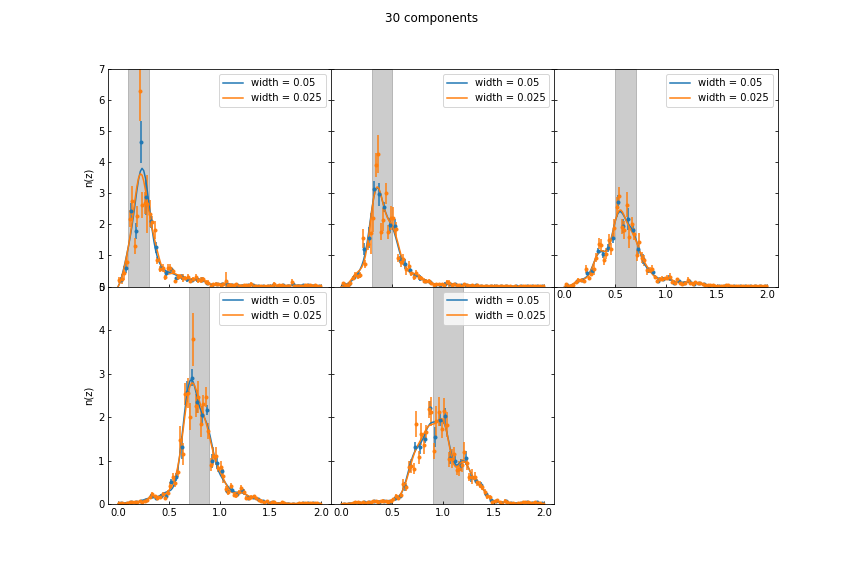
\includegraphics[scale=0.3]{plots/30.png}
\caption{Comparison of redshift distribution calibrated with input data histograms with bin width of $\Delta z = 0.05$ and $\Delta z = 0.025$ {\color{red} change legend!}}
\label{fig:comb}
\end{figure}
\begin{table}
\label{tab:redshift_calibration}
\begin{tabular}{lllll}
\hline
dataset & $N_{\rm model}$ & d.o.f. & $\chi^2/{\rm d.o.f.}$& $\chi^2/{\rm d.o.f.}$ (diagonal only)\\
\hline
KV-450 DIR&20&20&56&6.0\\
$\Delta z = 0.05$&30&10&90&9.4\\
$N_{\rm data} = 40$&40&0&n/d&n/d\\
\hline
KV-450 DIR&20&60&90&5.3\\
$\Delta z = 0.025$&30&50&91&5.6\\
$N_{\rm data} = 80$&40&40&113&7.0\\
&50&30&136&8.8\\
&60&20&199&12.6\\
&70&10&388&23.8\\
&80&0&n/d&n/d\\
\hline
\end{tabular}
\caption{Fit results of the redshift calibration for two different choices of histogram bin width of the input data. }
\end{table}
\section{KV450 likelihood sampling with comb model but without marginalisation}
\label{ap:kv450_likelihood}
In order to test if the fitted redshift distribution is capable of reproducing the results of the fiducial KV-450 analysis we sample the likelihood using the model to parametrise the redshift distribution, but without marginalisation over the uncertainty of nuisance parameters. To make a fair comparison of the two likelihoods we fix the nuisance parameters $\delta z_i$ of the KV-450 likelihood. Results of these fits are presented Table \ref{tab:consistency}, showing the constraints on cosmological and nuisance parameters. We find that constraints from both setups are fully consistent and therefore we conclude the the fitted redshift distribution can be used as an alternative to the fiducial redshift histograms.

\begin{figure}
\centering
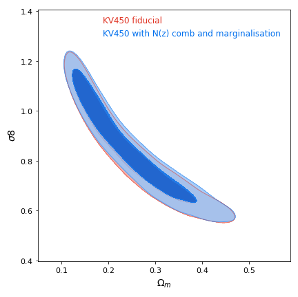
\includegraphics[scale=0.5]{plots/Om_s8.png}
\caption{{\color{red} This is a caption}}
\label{fig:Om_s8_consistency}
\end{figure}

\begin{table}
\begin{tabular}{lll}
\hline
\hline
Parameter & fiducial KV450 & KV450 with comb model\\
\hline
$\omega_{cdm }  $ & $0.112^{+0.029}_{-0.060}   $& $0.112^{+0.046}_{-0.060}   $\\

$\ln10^{10}A_{s }$ & $3.30\pm 0.92              $& $3.34\pm 0.92              $\\

$\omega_{b }    $ & $0.0223\pm 0.0021          $& $0.0222^{+0.0018}_{-0.0025}$\\

$n_{s }         $ & $1.03^{+0.15}_{-0.13}      $& $1.01\pm 0.13              $\\

$h              $ & $0.749^{+0.067}_{-0.028}   $& $0.746^{+0.062}_{-0.033}   $\\
\hline
$A_{IA }        $ & $0.89^{+0.64}_{-0.58}      $& $0.70^{+0.64}_{-0.58}              $\\

$c_{min }       $ & $2.50^{+0.22}_{-0.45}      $& $2.49^{+0.23}_{-0.40}     $\\

$dc             $ & $0.00000\pm 0.00019        $& $0.00000\pm 0.00019        $\\

$Ac             $ & $1.03\pm 0.12              $& $1.02\pm 0.12              $\\

$\Omega_{m }    $ & $0.242^{+0.052}_{-0.11}    $& $0.242^{+0.055}_{-0.11}    $\\

$\sigma_8        $ & $0.86^{+0.18}_{-0.20}      $& $0.87\pm 0.17      $\\
\hline
\end{tabular}
\caption{{\color{red} This is a caption}}
\label{tab:consistency}
\end{table}
\end{appendix}
%
%
\end{document}
